\subsubsection{Energy Awareness at Individual and Collective Levels}\label{sec:energydata}

This part of the application is designed and developed to enable an informed approach to ``fair energy use'' by making people aware of their
energy behaviors in individual and collective terms. Indeed, it includes means for users to visualize in an easily
understandable and actionable way a specific set of energy measurements, simple analytics and a time-of-use (ToU) signal.

The access point for this part of the app is the ``Energy Data'' navigation tab (Figure \ref{fig:tab}). This tab gives access to an
overview of the various functionalities and visualizations of specific information: ``Energy Meteo'', Visualization of consumption and production data (real time and historical),
``Comparisons'' data.

There are three main categories of information provided through this part of the app:
\begin{itemize}
 \item Time of use signal
 \item Visualization of real time and historical data (individual level)
 \item Comparative visualizations (collective level)
\end{itemize}

\begin{figure}[htb]
\centering
\frame{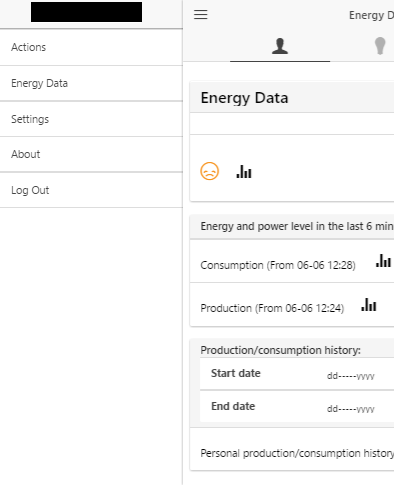
\includegraphics[width=0.5\linewidth]{img/trentinooverview_tab3.png}}
% 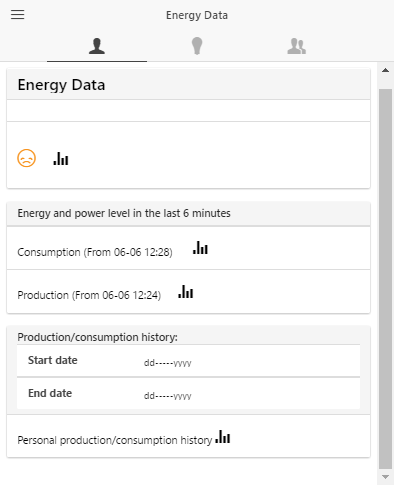
\includegraphics[width=0.33\linewidth]{img/trentinooverview3.png}
% 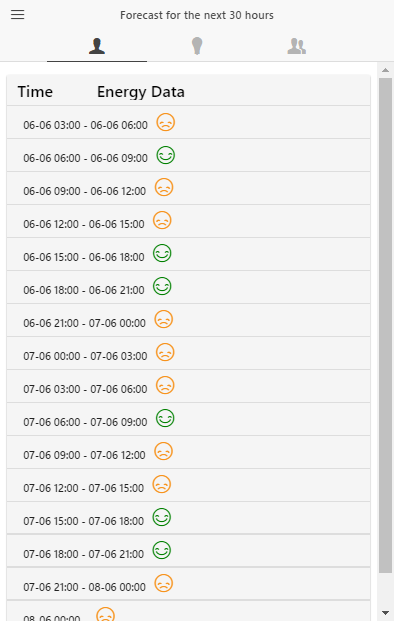
\includegraphics[width=0.307\linewidth]{img/touprediction.png}
\caption{Navigation tab with access to the feature for energy awareness: ``Energy Data''}\label{fig:tab}
\end{figure}

Although the direct impact of these kind of information can be debated -- reported reductions ranging from 2\% to 20+\% \citep{eea_report} and the fact the their medium and
long-term implications received some criticisms (with particular regards to normative ``eco-feedback''~\citep{Strengers2012,Cakici2014}), this part of the app is in-line with the needs emerged from
the pilot sites and the project activities\footnote{Requirements analyzed as reported in Deliverable 3.1. Design concept validated as reported in Deliverable 3.2.}.
It also addresses the fact that improvements of dwellers' energy awareness remain a necessary condition towards the long-term adoption of more sustainable behaviors,
although not sufficient alone. Indeed, this part of the app has been designed with broader processes of social change
in mind\footnote{For further details, see the User Story ``Energy Garden'' included in Deliverable 1.3.}. Therefore, ``energy awareness'' should be considered as instrumental to
well defined individual and collective efforts. 


\paragraph{``Energy Meteo'': the Time-of-Use (ToU) signal} 
It is designed to leverage load elasticity for maximizing self-consumption, with the twofold effect of optimizing usage of locally-installed RESs and minimizing dependency from energy markets. This means that electric loads shall be shifted to periods of time characterized by high local production from renewable energy sources.
It provides users with a clear indication of the actual status of the local grid: \textit{green smilies} signal slots when local production exceeds demand; \textit{red smilies} highlight slots
when demand exceeds local production\footnote{See Deliverable 4.2 \textbf{[NB: VERIFY!!]}, for more details on the technical design and implementation of the predictive model of the ToU signal.}.

\begin{figure}[htb]
      \begin{center}
        \begin{minipage}[htb]{0.45\linewidth}    
         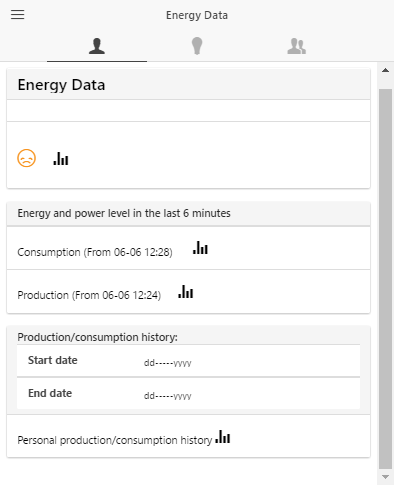
\includegraphics[width=1\linewidth]{img/trentinooverview3.png}   
         \vspace{1.9cm}
        \end{minipage}
% 	\hfill 
        \begin{minipage}[htb]{0.45\linewidth}    
         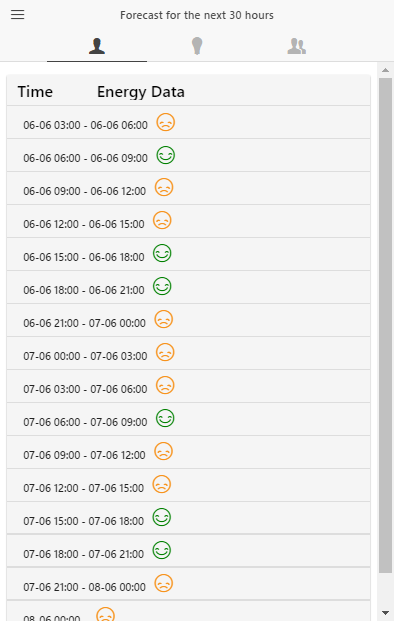
\includegraphics[width=1\linewidth]{img/touprediction.png}   
        \end{minipage}
      \end{center}
      \caption{(1) ``Energy Data'' main screen: overview of the various functionalities and easy access to visualization of specific information;
(2) ToU signals with a 30-hours forecast, divided by 3-hours slots.}\label{fig:overview-tou}
\end{figure}

The ToU signal is provided in two distinct ways:
\begin{description}
 \item[Current.] It is available on the main screen (Figure \ref{fig:overview-tou}-1) and it indicates whether \textit{present} moment is a good (`green smiley') or bad moment (`red smiley')
 to consume locally produced electricity.
 \item[Forecast.] It is available by clicking on ``Energy Meteo'' field and it provides a detailed overview of the local grid conditions, forecasted in 3-hours time-slots, for the forthcoming 30 hours (Figure \ref{fig:overview-tou}-2). A new forecast is generated every 24 hours.
\end{description}



\paragraph{Visualization of consumption and production (real time)} 
It is designed to inform users about their (near to) real time electric consumption and (where available) production data.
\begin{figure}[htb]
      \begin{center}
        \begin{minipage}[htb]{0.45\linewidth}    
         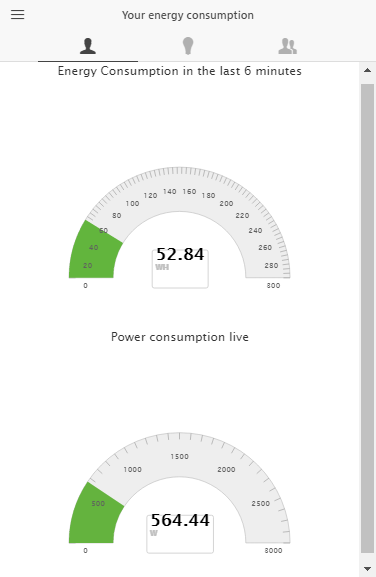
\includegraphics[width=1\linewidth]{img/visual_consumption.png}  
        \end{minipage}
% 	\hfill 
        \begin{minipage}[htb]{0.45\linewidth}    
         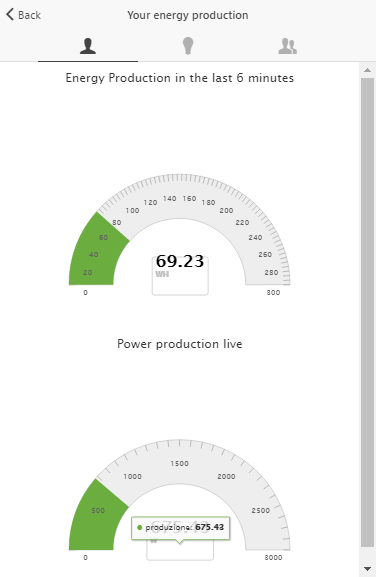
\includegraphics[width=1\linewidth]{img/visual_production.png}  
        \end{minipage}
      \end{center}
    \caption{(1) Energy and Power meters for household's electric consumption measurements; (2) Energy and Power meters for household's electric production measurements.
}
\label{fig:viz_rt}
\end{figure}

Users can access these information from the ``Energy Data'' main screen and either visualize the household's electric consumption (Figure \ref{fig:viz_rt}-1) or
household's electric production (Figure \ref{fig:viz_rt}-2).
These visualizations provide meters for:
\begin{description}
 \item[Energy.] It is accounted for the most recent 6-10 minutes monitored.
 \item[Power.] It provides instant measurement\footnote{For technical reasons and depending on several environmental factors (\textit{e.g.} households connectivity for transfer of monitored data) there may be up to approximately 2 minutes delay between the actual power measured and the data displayed through You Power.}.
\end{description}



\paragraph{Visualization of historical data} 

This feature is designed to provide users with a broader temporal overview on their energy habits.
\begin{figure}[htb]
      \begin{center}
        \begin{minipage}[htb]{0.45\linewidth}    
         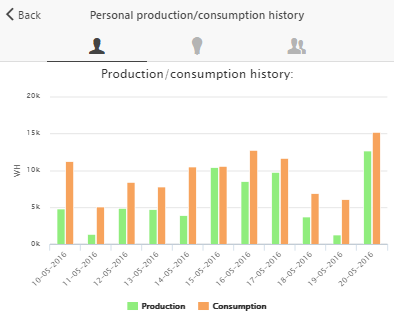
\includegraphics[width=1\linewidth]{img/historicalcomparison_prodcons.png}
        \end{minipage}
% 	\hfill 
        \begin{minipage}[htb]{0.45\linewidth}    
         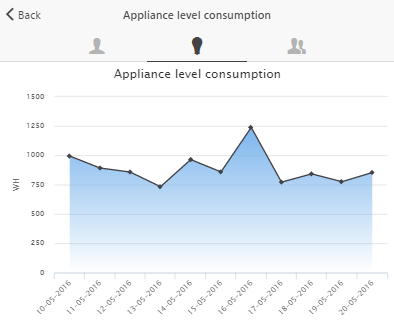
\includegraphics[width=1\linewidth]{img/applianceconsumption.png}
        \end{minipage}
      \end{center}
      \caption{(1) Household overview of electric energy consumption and production, for the chosen data range; (2) Consumption patterns for the chosen data range at appliance level.
}
\label{fig:viz_hist}
\end{figure}

Information about historical data are available both for household and appliance levels:
\begin{description}
 \item[Household.] It provides a daily overview of the overall electric energy consumption and production for the chosen data range. This shall give a basis for dwellers to understand and improve their self-consumption.
 \item[Appliance.] It provides a detailed view of the consumption patterns for the selected appliance. Visualized appliances are the ones equipped with smart plugs. 
\end{description}
Selection of data ranges are mandatory for these visualizations. They must be set by users at two different places: in the ``Energy Data'' main screen for the \textit{Household} category;
in the `light-bulb' sub-view for the \textit{Appliance} one, which is accessible from the top level bar.


\paragraph{Visualization of comparisons} 
Comparisons are designed to provide users with reference information about energy performances or behaviors in relation to the neighborhoods.
\begin{figure}[htb]
      \begin{center}
        \begin{minipage}[htb]{0.45\linewidth}    
         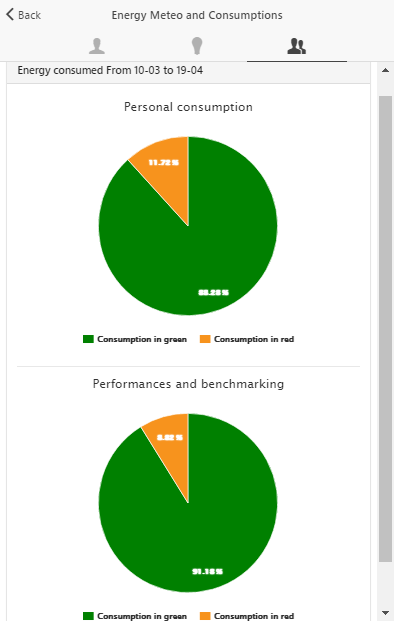
\includegraphics[width=1\linewidth]{img/touperformancechart_indivcoll.png}
        \end{minipage}
% 	\hfill 
         \begin{minipage}[htb]{0.45\linewidth}    
         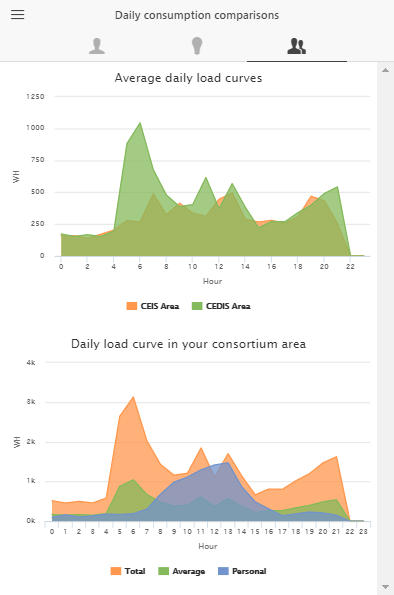
\includegraphics[width=1\linewidth]{img/benchmark.png}
        \end{minipage}
      \end{center}
      \caption{(1) Compares individual consumption with community one with regards to the distribution between the delivered ToU signals; (2) Shows the average consumption load curves at the level of the two Consortia and compares the individual curve with the average and the total of the related Consortium area.
}
\label{fig:comparison}
\end{figure}
There are two type of comparisons that can be visualized through YouPower:
\begin{description}
 \item[Consumption distribution on ToU signals] It shows a cumulative and progressive distribution of consumption between the green and red ToU signals.
 On the top part it shows the individual household chart, while on the bottom, the community\footnote{In this case community refers to the registered users who 
 are served by the same Energy cooperative through the same local distribution network.} total distribution. This view is a static one and is progressively updated on a weekly basis. The descriptive label for the chart clearly highlights the reference period considered.
 \item[Consumption profile benchmark] It provides users with a benchmark\footnote{While in principle homogeneous groups of users could be identified to make the comparison more sound, this requires data (household composition, size of dwelling, type and number of appliances preset, thermal isolation \ldots) which are not currently available for the vast majority of the users engaged in the pilot.
 Furthermore, the heterogeneity and limited number of users involved would not allow to form meaningful groups for creating sound averages and benchmarking. For this reason the simple community average is used as a benchmark.} of consumption profile -- \textit{load curve}. It provides two graphs. At the top part of the screen the load curves are shown as average of households enrolled by the two Consortia.
 At the bottom part, household's load curve is compared with the average and the total of the related Consortium. These information are available only at a daily level. Therefore, users have to select the day (available starting from the previous day and backwards) for which they want to visualize such benchmarks
\end{description}
These features can be accessed by clicking on the ``community'' icon, which is symbolized by the two people on the top level bar.


\paragraph{Participatory Budgeting external service} 

This external service\footnote{This service was initially expected to be integrated in YouPower. However, due to the delays for the app deployment it was not possible
to fully develop and integrate it in YouPower. Therefore, similar functionalities have been provided through
this external service.} and process is designed to accompany users along their efforts of changing their energy behaviors.
In particular, it supports the objective to maximize the use of locally produced electricity\footnote{The full narrative behind this type of energy intervention
is described in CIVIS Deliverable 1.3}, by means of a collective deliberation process for the allocation of an `energy bonus', which is collected through the consumptions
made under the green ToU signal.

A website has been implemented to:
\begin{itemize}
 \item detail the conditions and regulations for the participatory budgeting process;
 \item submit idea proposals for the awarding of the ``energy bonus'';
 \item update involved users about the proposals received;
 \item inform users about the various steps along the evaluation and selection procedures for the awarded proposals. 
\end{itemize}
The website can be reached at \url{https://progettocivis.wordpress.com/}.

%